% Drawing 148/02-14 -- folder 148, batch 02, archive page 33 (PDF page 34).
% Transcription: à droite, une sphère : un pôle marqué en haut et quatre points sur l'équateur, deux à l'avant et deux à l'arrière (en tirets).
% Kind: sphere with one pole and four points on the equator. Method 2 (schematic redraw from the facsimile). Status: ok.
% Notes: Ink. The outline, a dot at the top (the pole, placed on the outline), the equator with its front arc solid and its back arc dashed, two dots on each. Redrawn 2026-11-12 (issue 128): to check again.
% Coordinates: 1 unit = 1 mm = 1/100 of the crop width, y downwards as on the crop (bbox in page fractions: [0.74, 0.535, 0.88, 0.6]).
% Redrawn by Claude (claude-fable-5-2), issue #128, 2026-11-12; not checked by a human; not compiled (no TeX in the session).
% Rights: reproduces part of the work -- behind RENDER_TRANSCRIPTS, never published by itself.
\documentclass[tikz,border=3pt]{standalone}
\usepackage{amsmath,amssymb}
\usetikzlibrary{patterns,arrows.meta}
\tikzset{pencil/.style={black!45}, struck/.style={black!35}, mpt/.style={circle,draw,inner sep=1.3pt}, pt/.style={circle,fill,inner sep=0.9pt}, opt/.style={circle,draw,fill=white,inner sep=1.1pt}, Rd/.style={red!75!black}, Gn/.style={green!45!black}, Br/.style={brown!70!black}}
\begin{document}
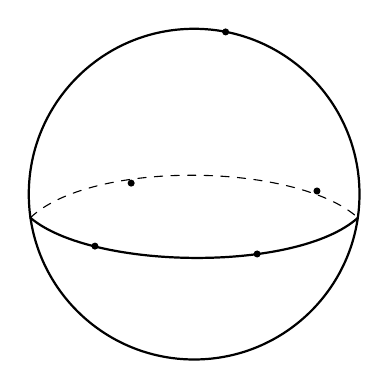
\begin{tikzpicture}[x=1mm,y=-1mm,line cap=round,line join=round,font=\small]
\draw[thick] (43,30) circle [radius=21];
\node[pt] at (47,9.4) {};
\draw[thick] (22.2,33) .. controls (30,39.6) and (56,40) .. (63.8,33);
\draw[dashed] (22.2,33) .. controls (30,25.6) and (56,26) .. (63.8,33);
\node[pt] at (30.4,36.6) {};
\node[pt] at (51,37.6) {};
\node[pt] at (35,28.6) {};
\node[pt] at (58.6,29.6) {};
\end{tikzpicture}
\end{document}
